\documentclass{article}
\usepackage[utf8]{inputenc}

\title{Tarea 2 Graficación de palabras y letras}
\author{Rómulo Enrique Troncoso Pacheco}
\date{September 2020}

\usepackage{natbib}
\usepackage{graphicx}

\begin{document}


\maketitle

\section{Introducción}
El ploteo es una práctica comúnmente utilizada en revistas científicas, libros y materiales impresos, que sirven al lector para poder identificar de forma visual en forma de gráficas datos con mayor sencillez y comprensión en la exposición de elementos evaluados. Esto, genera la posibilidad de establecer estadísticas con fines comparativos relacionados a la identificación de cantidades  de letras y palabras que se puedan presentar en índices numéricos.

De esta forma, en esta práctica académica se establecen letras y palabras que mantienen una mayor frecuencia en el libro de The King in Yellow by Robert W. Chambers\cite{The_King_in_Yellow}, con la finalidad de generar un ejercicio de graficación de frecuencias en términos numéricos.
La importancia del ploteo es el establecer fundamentos para realizar un análisis de datos con la finalidad de emplearlo en diversas ramas de las ciencias. De esta forma, esta práctica se orienta a una serie de pasos en los cuales se ejecutaron de forma sistemática mediante instrucciones específicas incluyendo siete apartados donde se describe la secuencia a seguir para la utilización del lenguaje de programación utilizado R\cite{r}.

\section{Herramientas de desarrollo}
Dentro de la práctica se utilizaron lenguajes de programación, librerías y editores de textos que consistieron en:

Lenguaje de programación R\cite{r}: utilizado para el enfoque de análisis estadístico originado desde los cimientos del lenguaje S; cuya finalidad, era convertir ideas en software de forma rápida y fiel, por ello, se generó las instrucciones que llevan una secuencia y lógica de pasos para cumplir algún objetivo en específico, como lo es el ploteo como instrucción.

Librerías: utilizado mediante un método de “librería” que consistente en fragmento de códigos, con el fin de facilitar las tareas al usuario para realizar una tarea en específico, para esta práctica se utilizaron las siguientes como gutenbergr\cite{gutenberg}, tidytext\cite{tidytext} y dplyr\cite{dplyr}.

Editores de texto: utilizado el Visual studio code\cite{Visual_studio_code}, que ayuda a plantear el manejo del texto del scrip. 

\section{Metodología}
En la práctica se describen las palabras con mayor impacto en el libro mencionado con antelación, con la finalidad de realizar una descripción exacta de elementos, relacionado de forma sistemática de acuerdo a la técnica de filtrado que auxilió  a concretar elementos exactos descriptivos en función a las letras y palabras del libro analizado.

Para ello, se utilizó las gráficas de barras como herrramienta de ploteo que permitió establecer la altura de cada una, en función a la proporción de la frecuencia obtenida del elemento estudiado.

\section{Objetivo}
Representar gráficamente las frecuencias de palabras y letras en el libro The King in Yellow by Robert W. Chambers\cite{The_King_in_Yellow}.
\subsection{Objetivo específico}
Graficar palabras y letras filtradas relacionadas a la frecuencia del libro The King in Yellow by Robert W. Chambers\cite{The_King_in_Yellow}.

\section{Procedimiento}
Para poder llevar a cabo el objetivo planteado de la práctica fue necesario realizar lo siguiente de acuerdo a las herramientas mencinadas anteriormente:
\begin{itemize}
    \item Cargar el libro.
    \item Separar palabras y letras.
    \item Graficar palabras.
    \item Graficar palabras filtradas.
    \item Graficar letras.
    \item Graficar letras filtradas.
\end{itemize} 
\section{Conclusión}
1.- Se pudo graficar las frecuencias relacionadas a las palabras y letras del libro analizado, referido en la sección de salida.

2.- Se pudo especificar de acuerdo a las herramientas y técnicas utilizadas la función de graficación para identificar las apartados correspondientes de palabras y letras repetidas con mayor frecuencia en el libro analizado.

3.- Relacionado al ploteo de las frecuencias de letras la "e" es la que tiene mayor frecuencia y la menor corresponde a la letra "z", señalando que el número con menor frecuencia corresponde al "6".

4.- Se pudo identificar mediante la base de datos que la palabra con mayor frecuencia corresponde a "the", como se observa en la figura 3  y con la menor frecuencia  la palabra "yell".


\section{Salida}
En esta sección se muestran las salidas del sistema donde se incluyen las siguientes gráficas:
\begin{figure}[ht]
    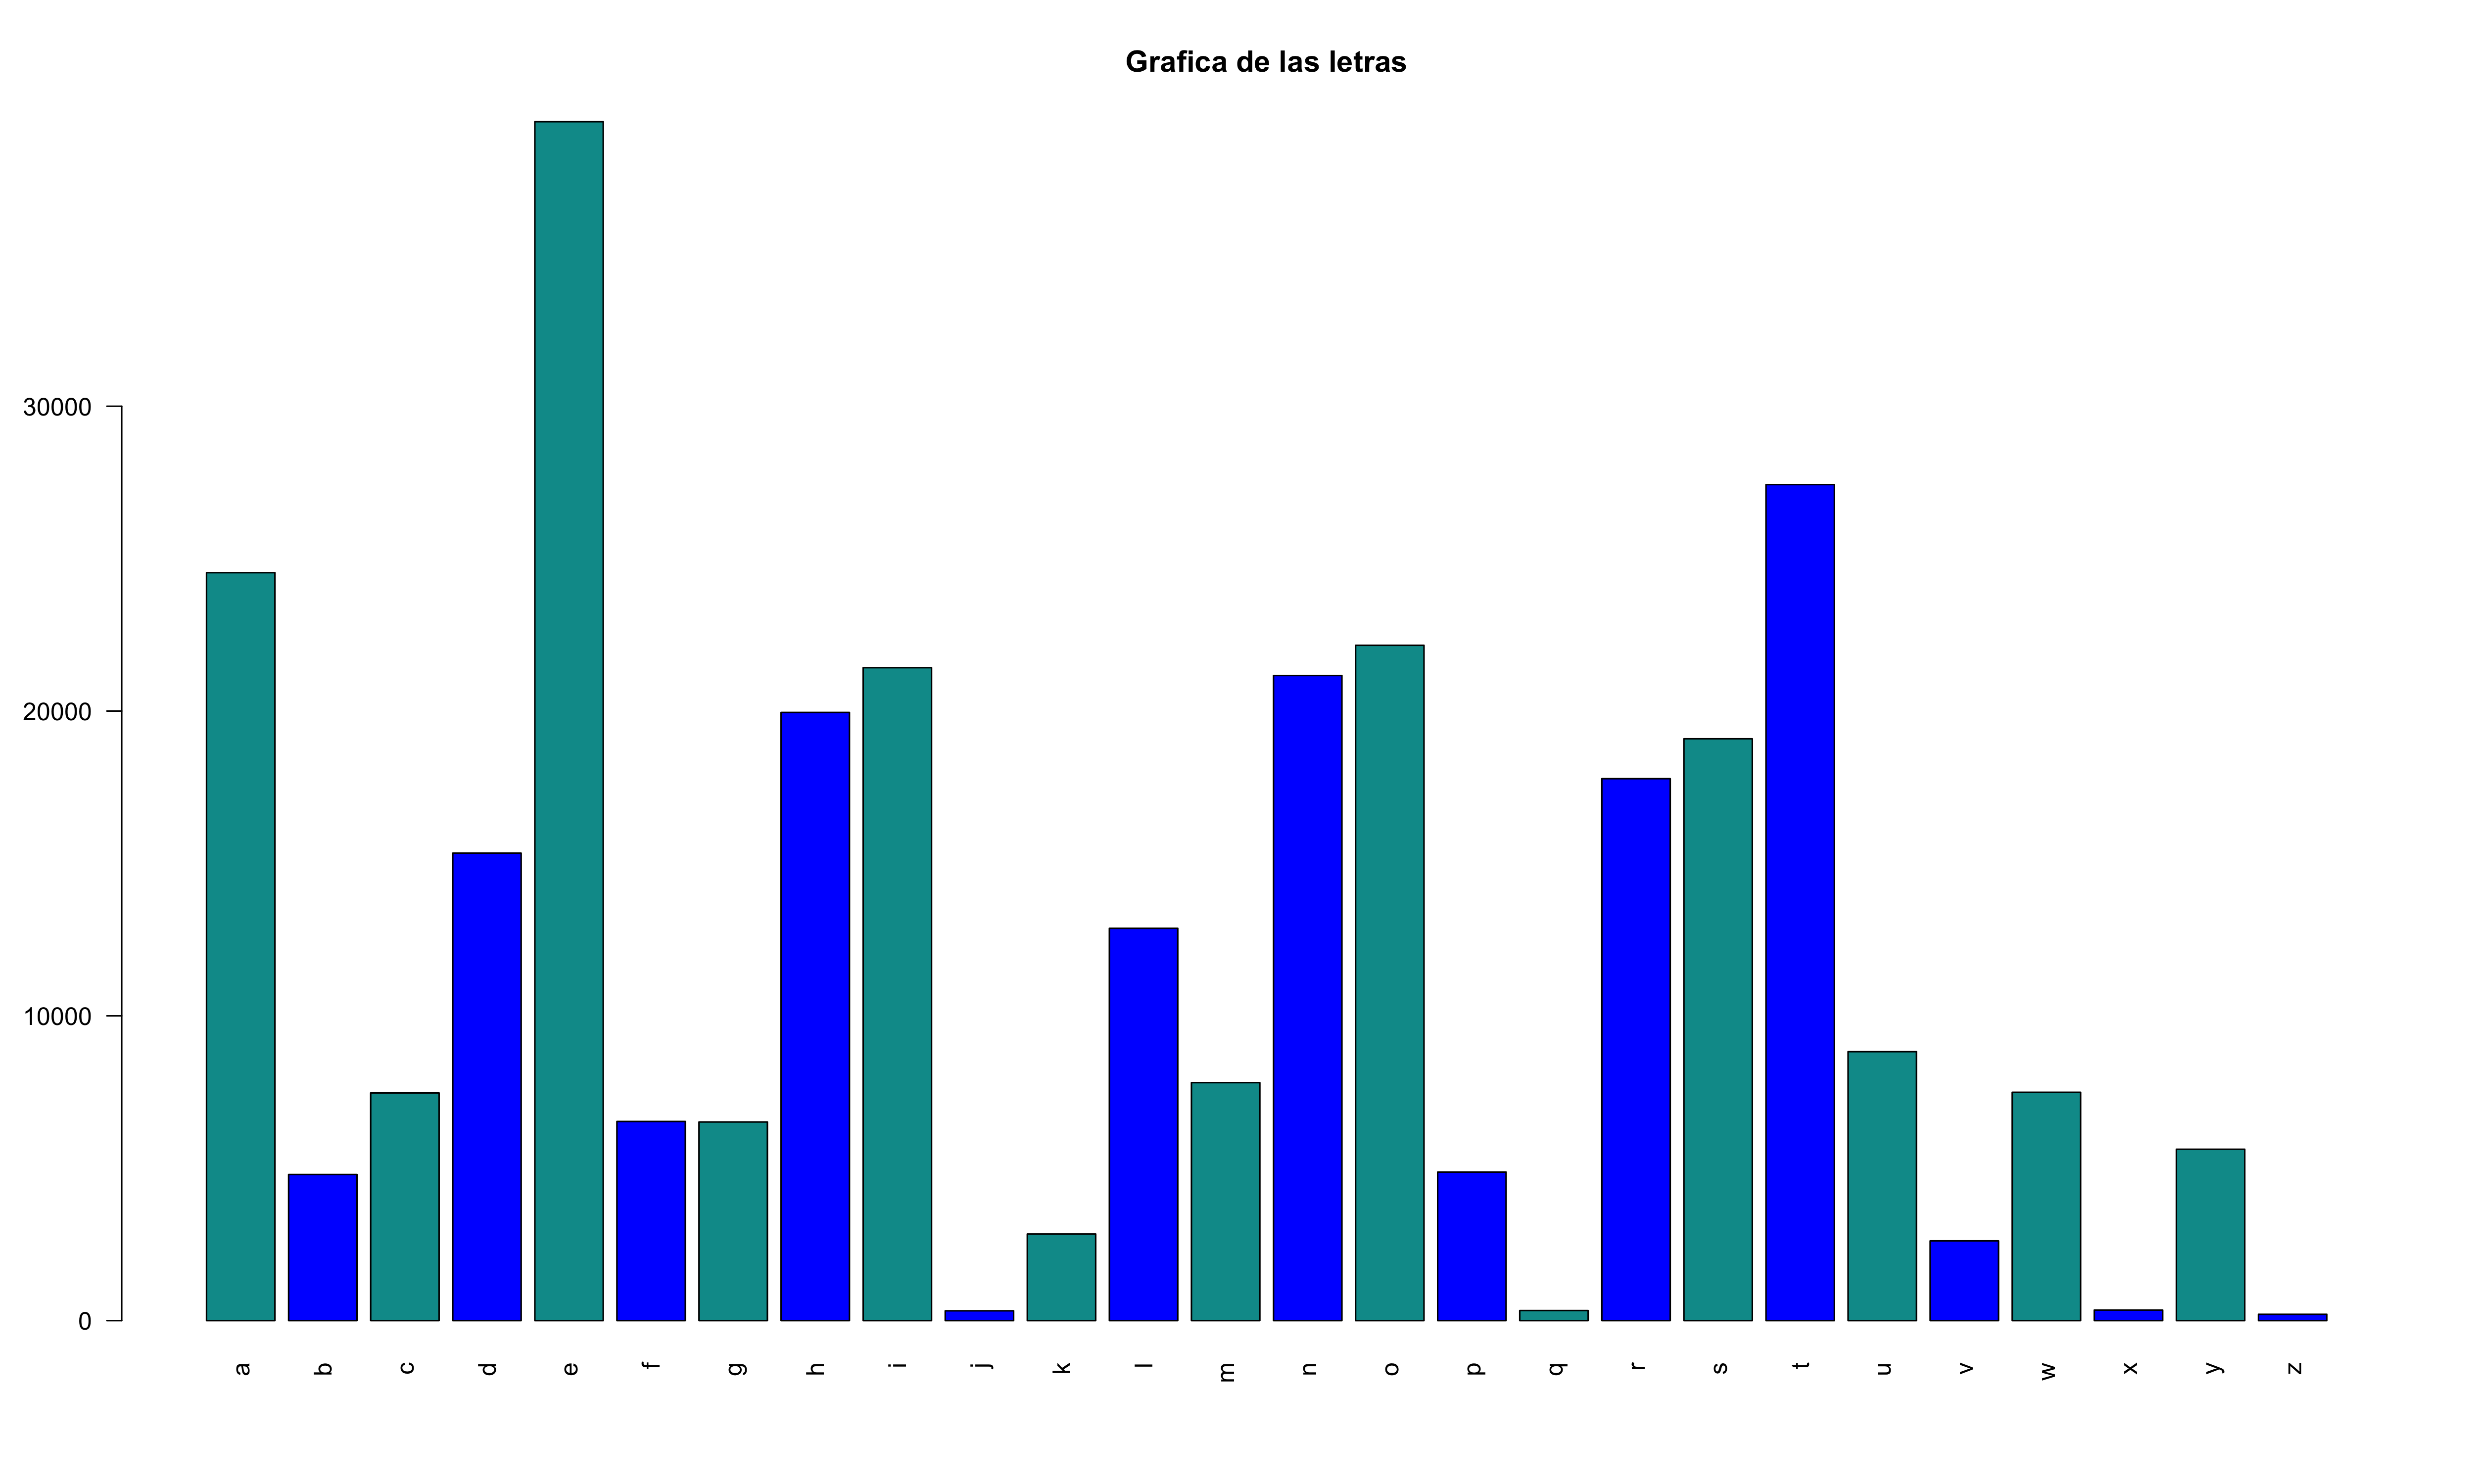
\includegraphics[scale=0.09]{Gráfica_de_las_letras.png}
    \caption{En esta gráfica se expone todas las letras utilizadas en el libro, con establecimiento de rango superior a 100 sin ordenamiento.}
    \label{fig:letras}
\end{figure}
\begin{figure}[ht]
    \centering
    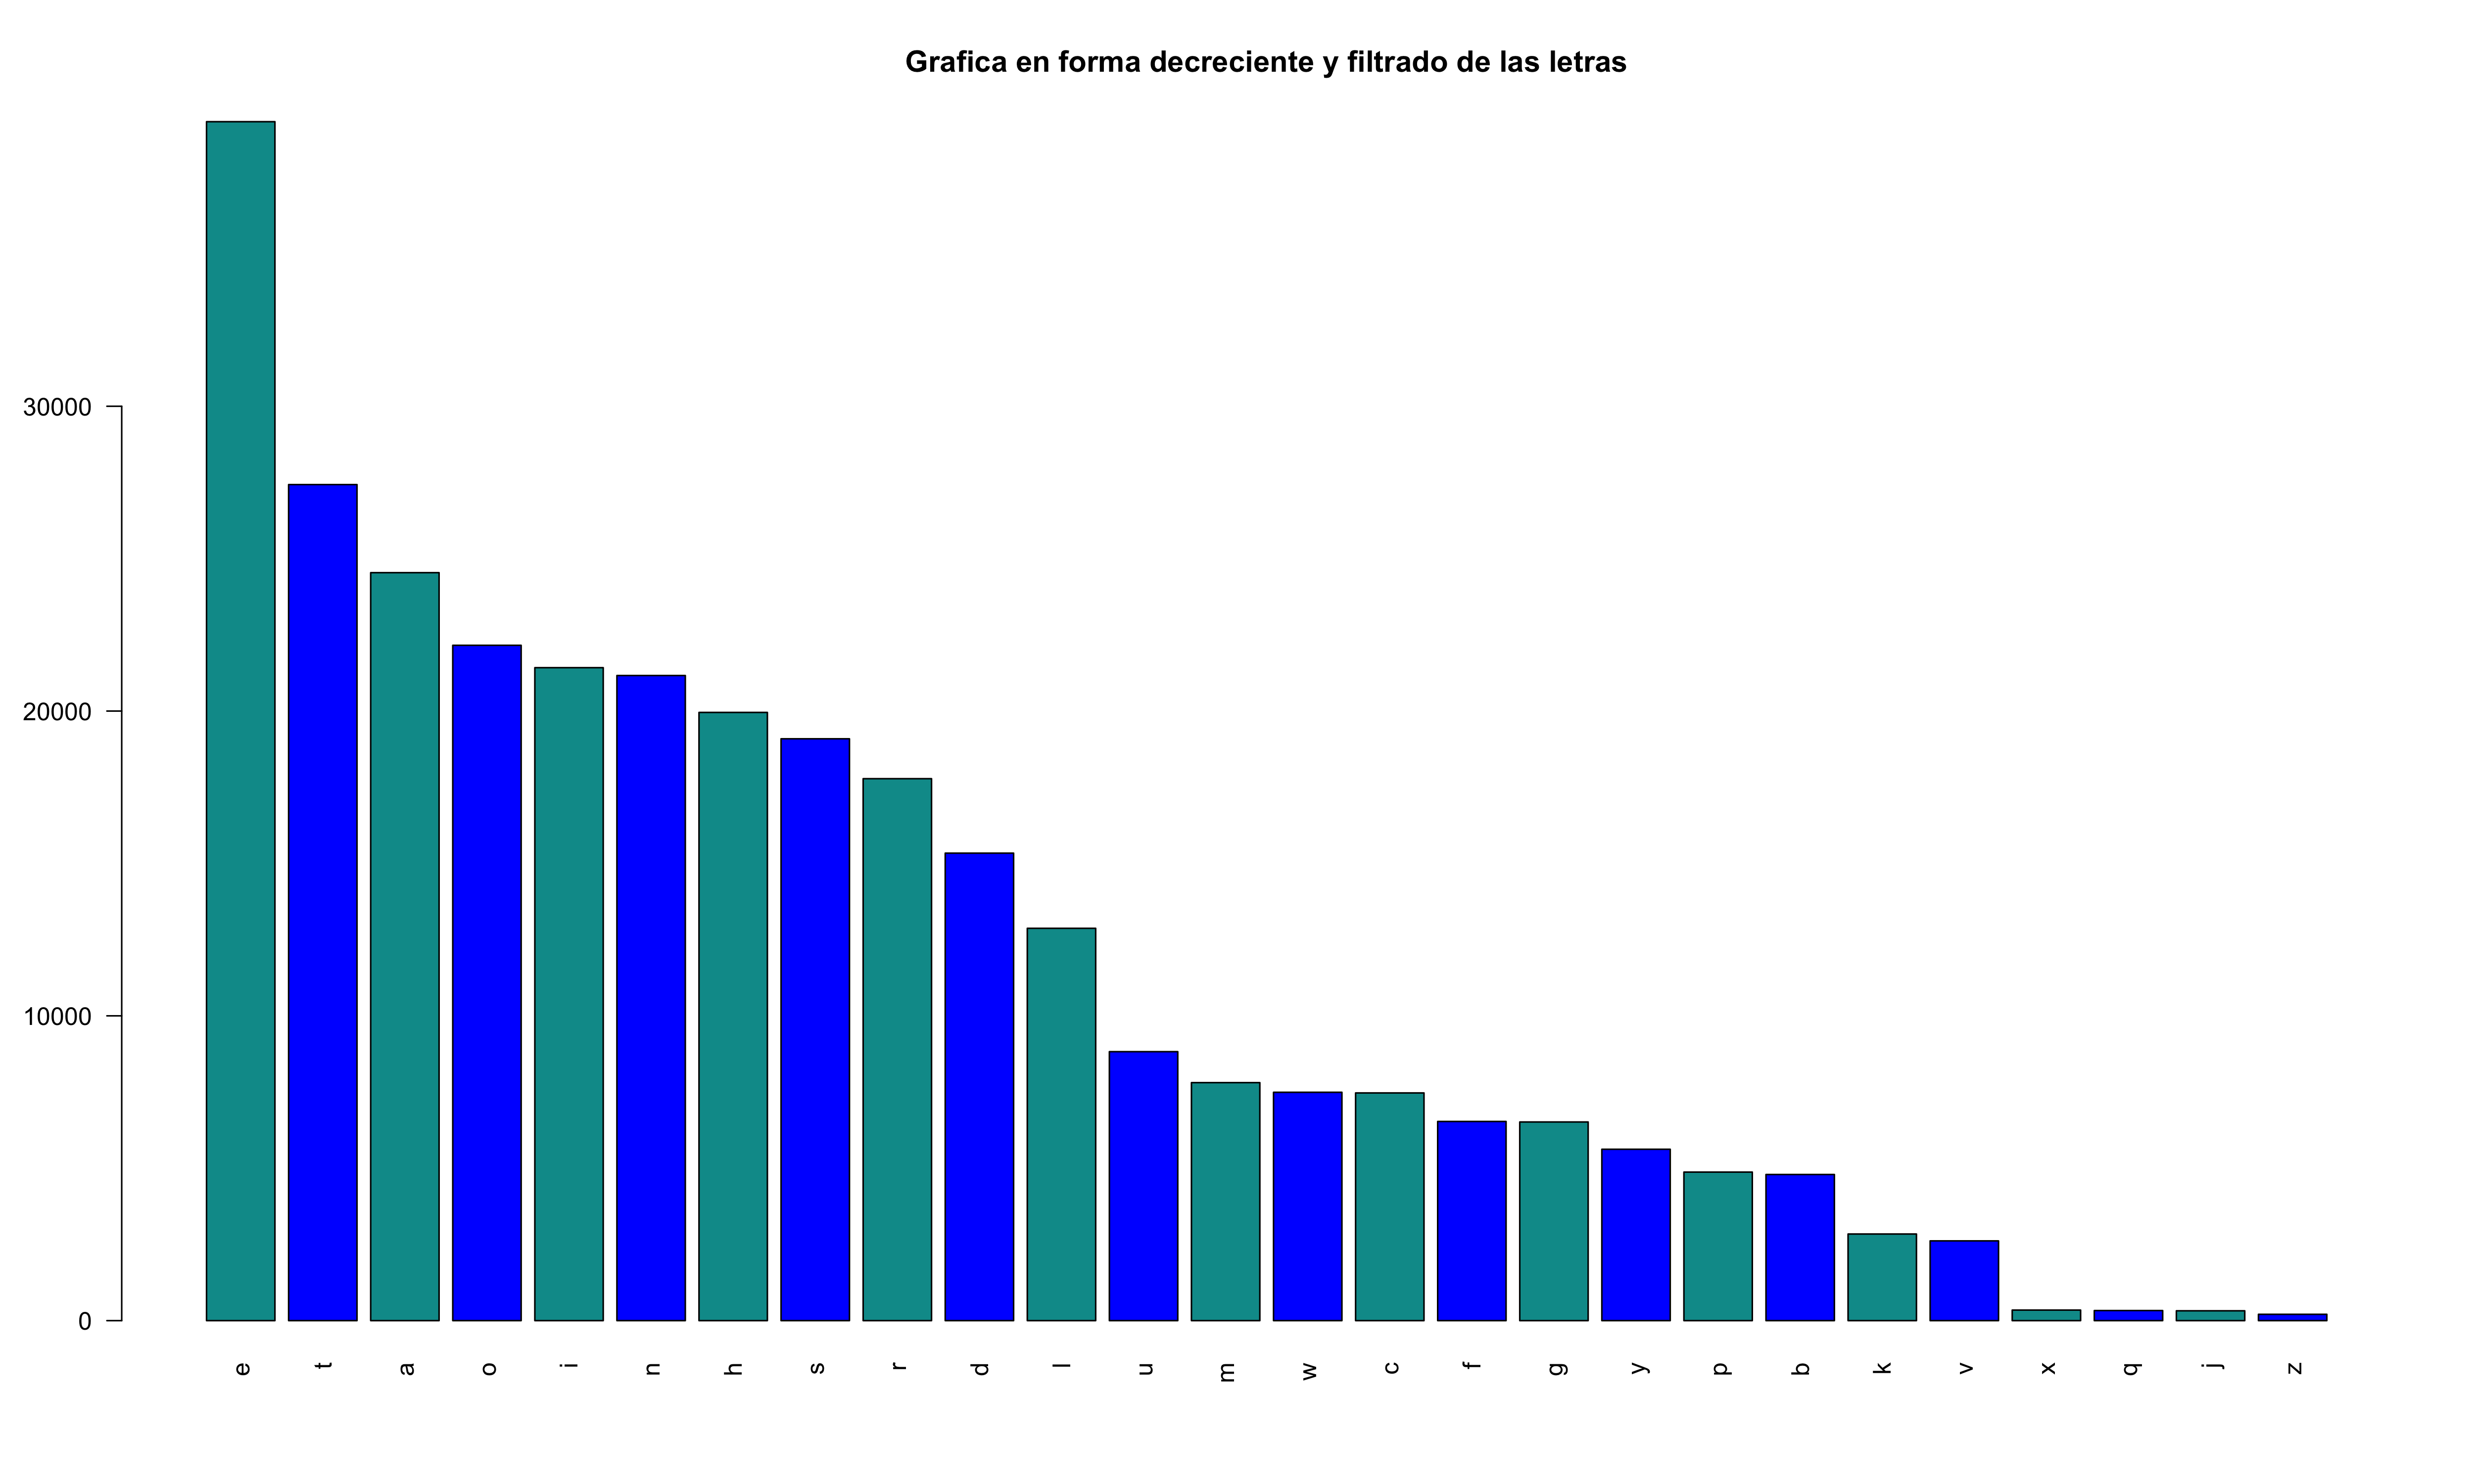
\includegraphics[scale=0.09]{Gráfica_en_forma_decreciente_y_filtrado_de_las_letras.png}
    \caption{En esta gráfica se expone las letras de forma decreciente en rangos superior a 100 }
    \label{fig:Letras_filtradas}
\end{figure}
\begin{figure}[ht]
    \centering
    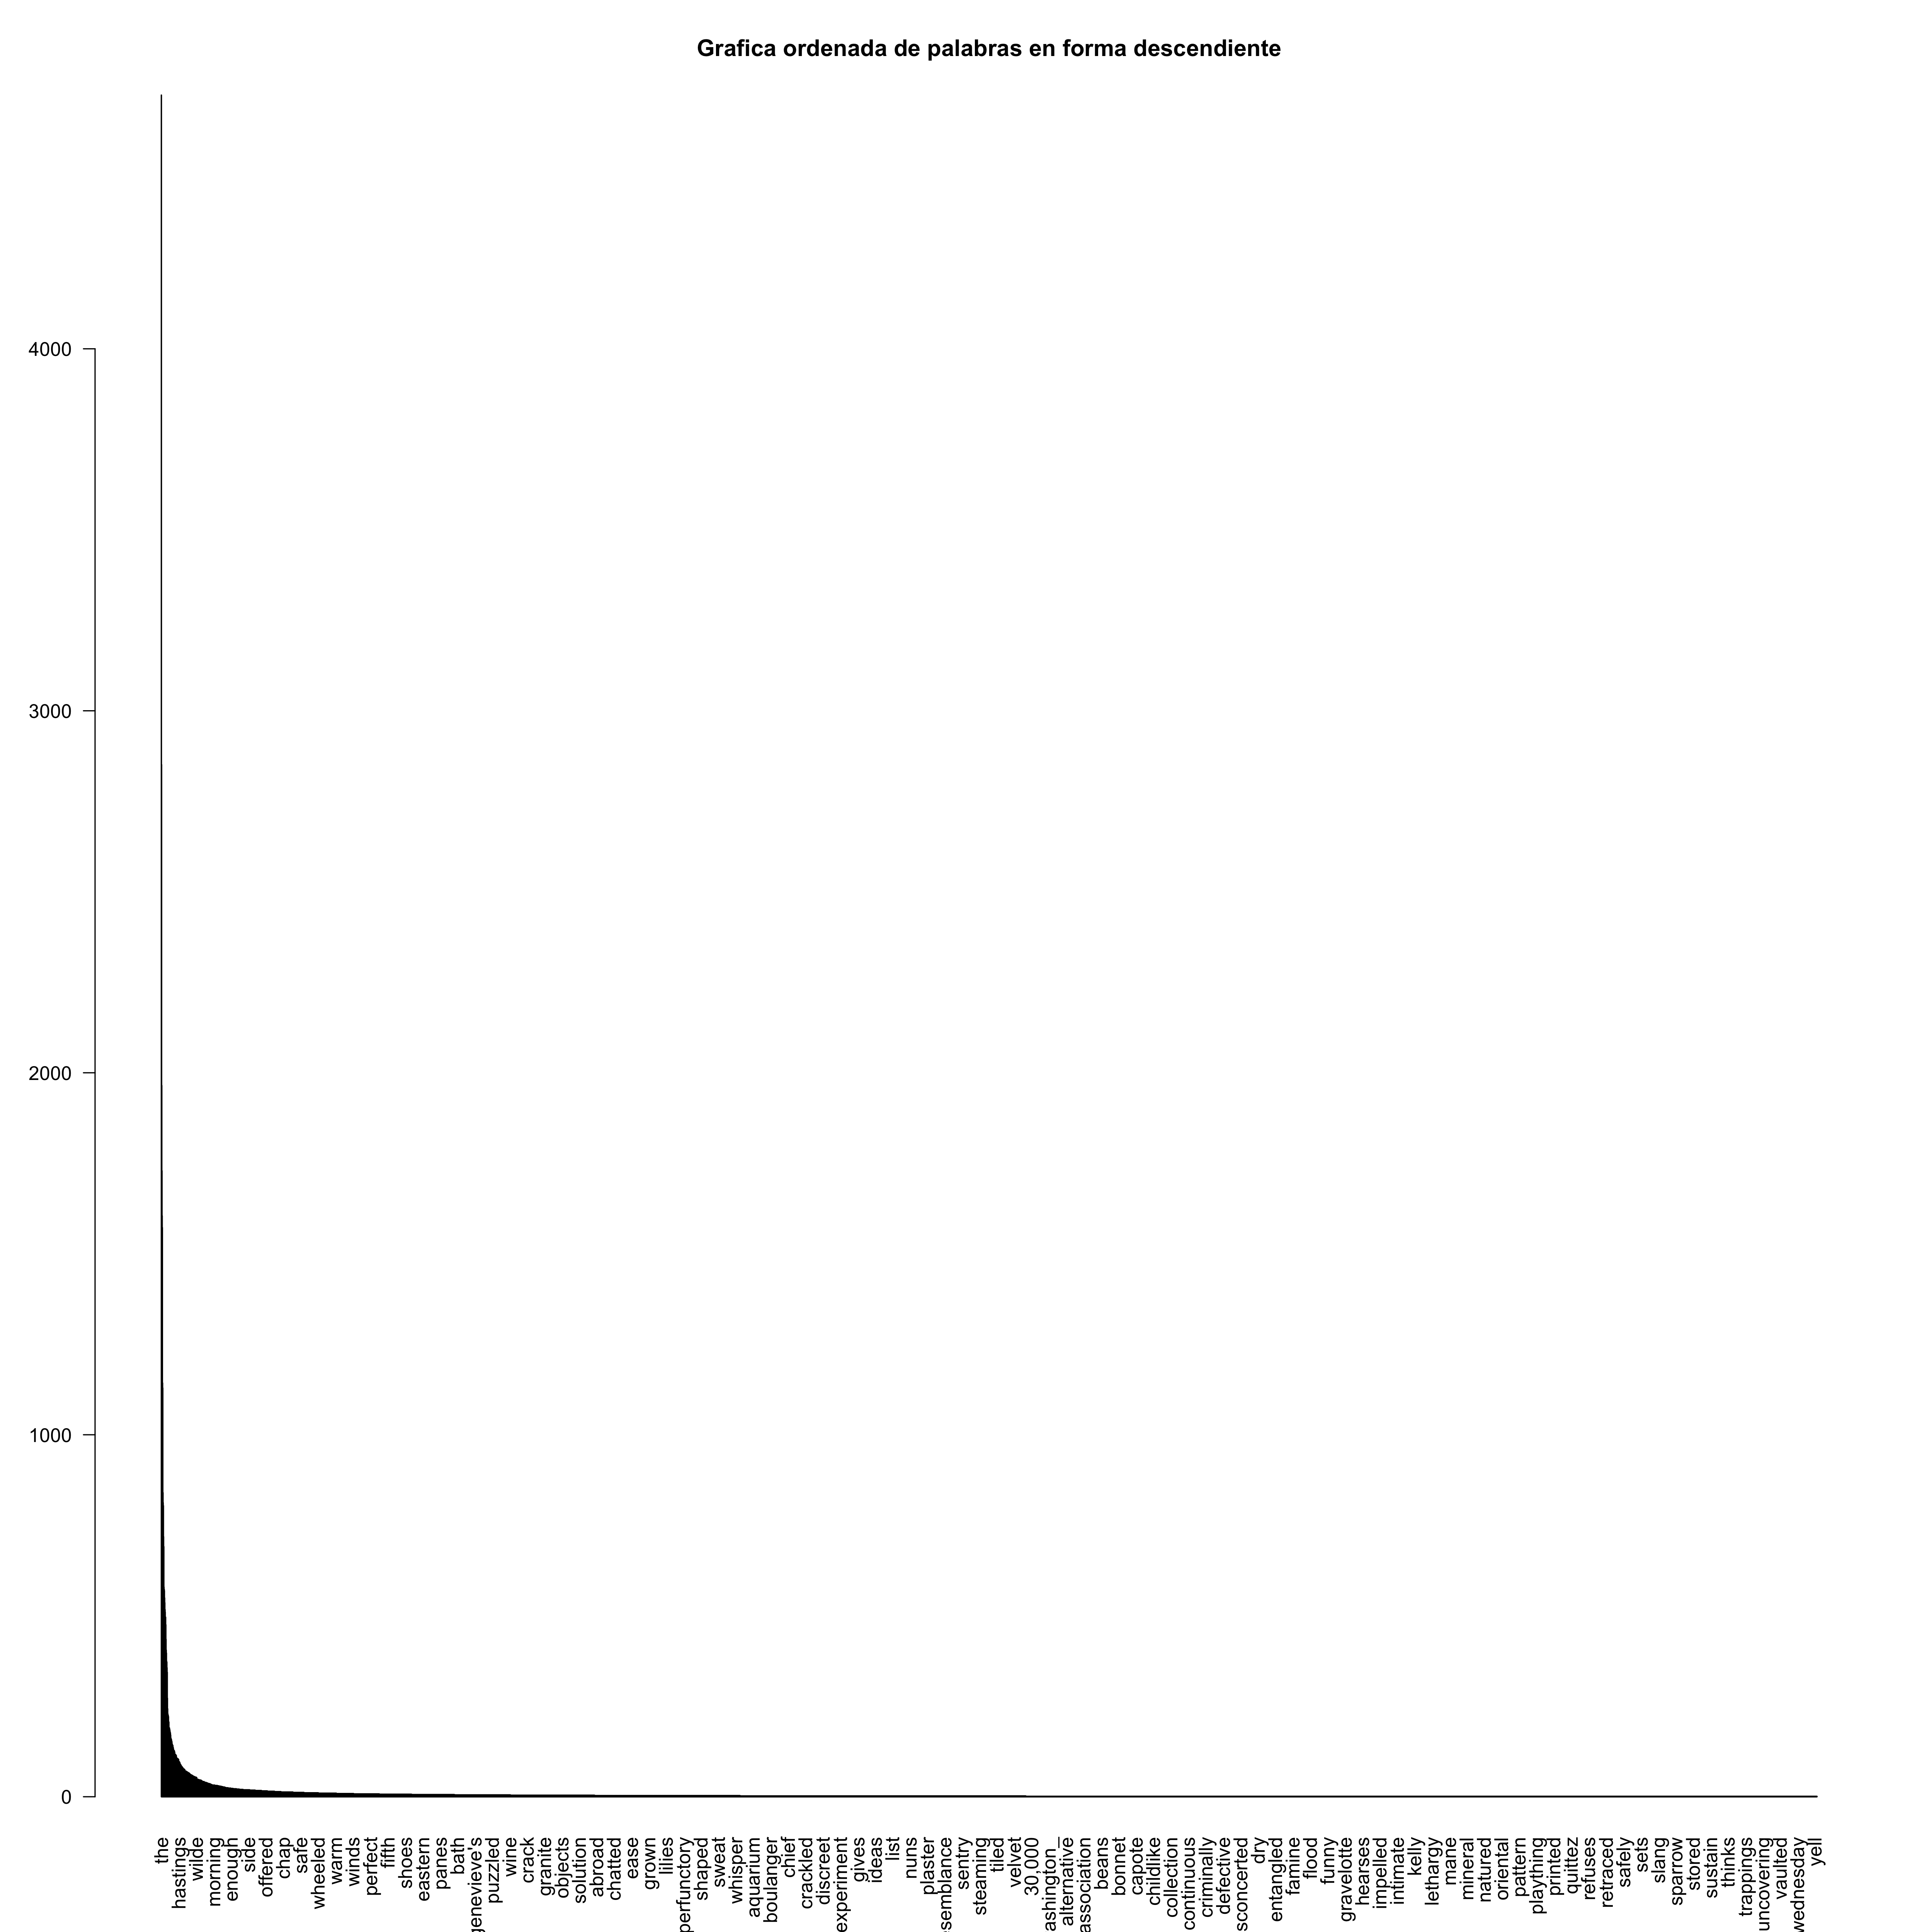
\includegraphics[scale=0.09]{Gráfico_Decreciente.png}
    \caption{En esta gráfica se expone todas las palabras en orden descendiente.}
    \label{fig:Palabras}
\end{figure}
\begin{figure}[ht]
    \centering
    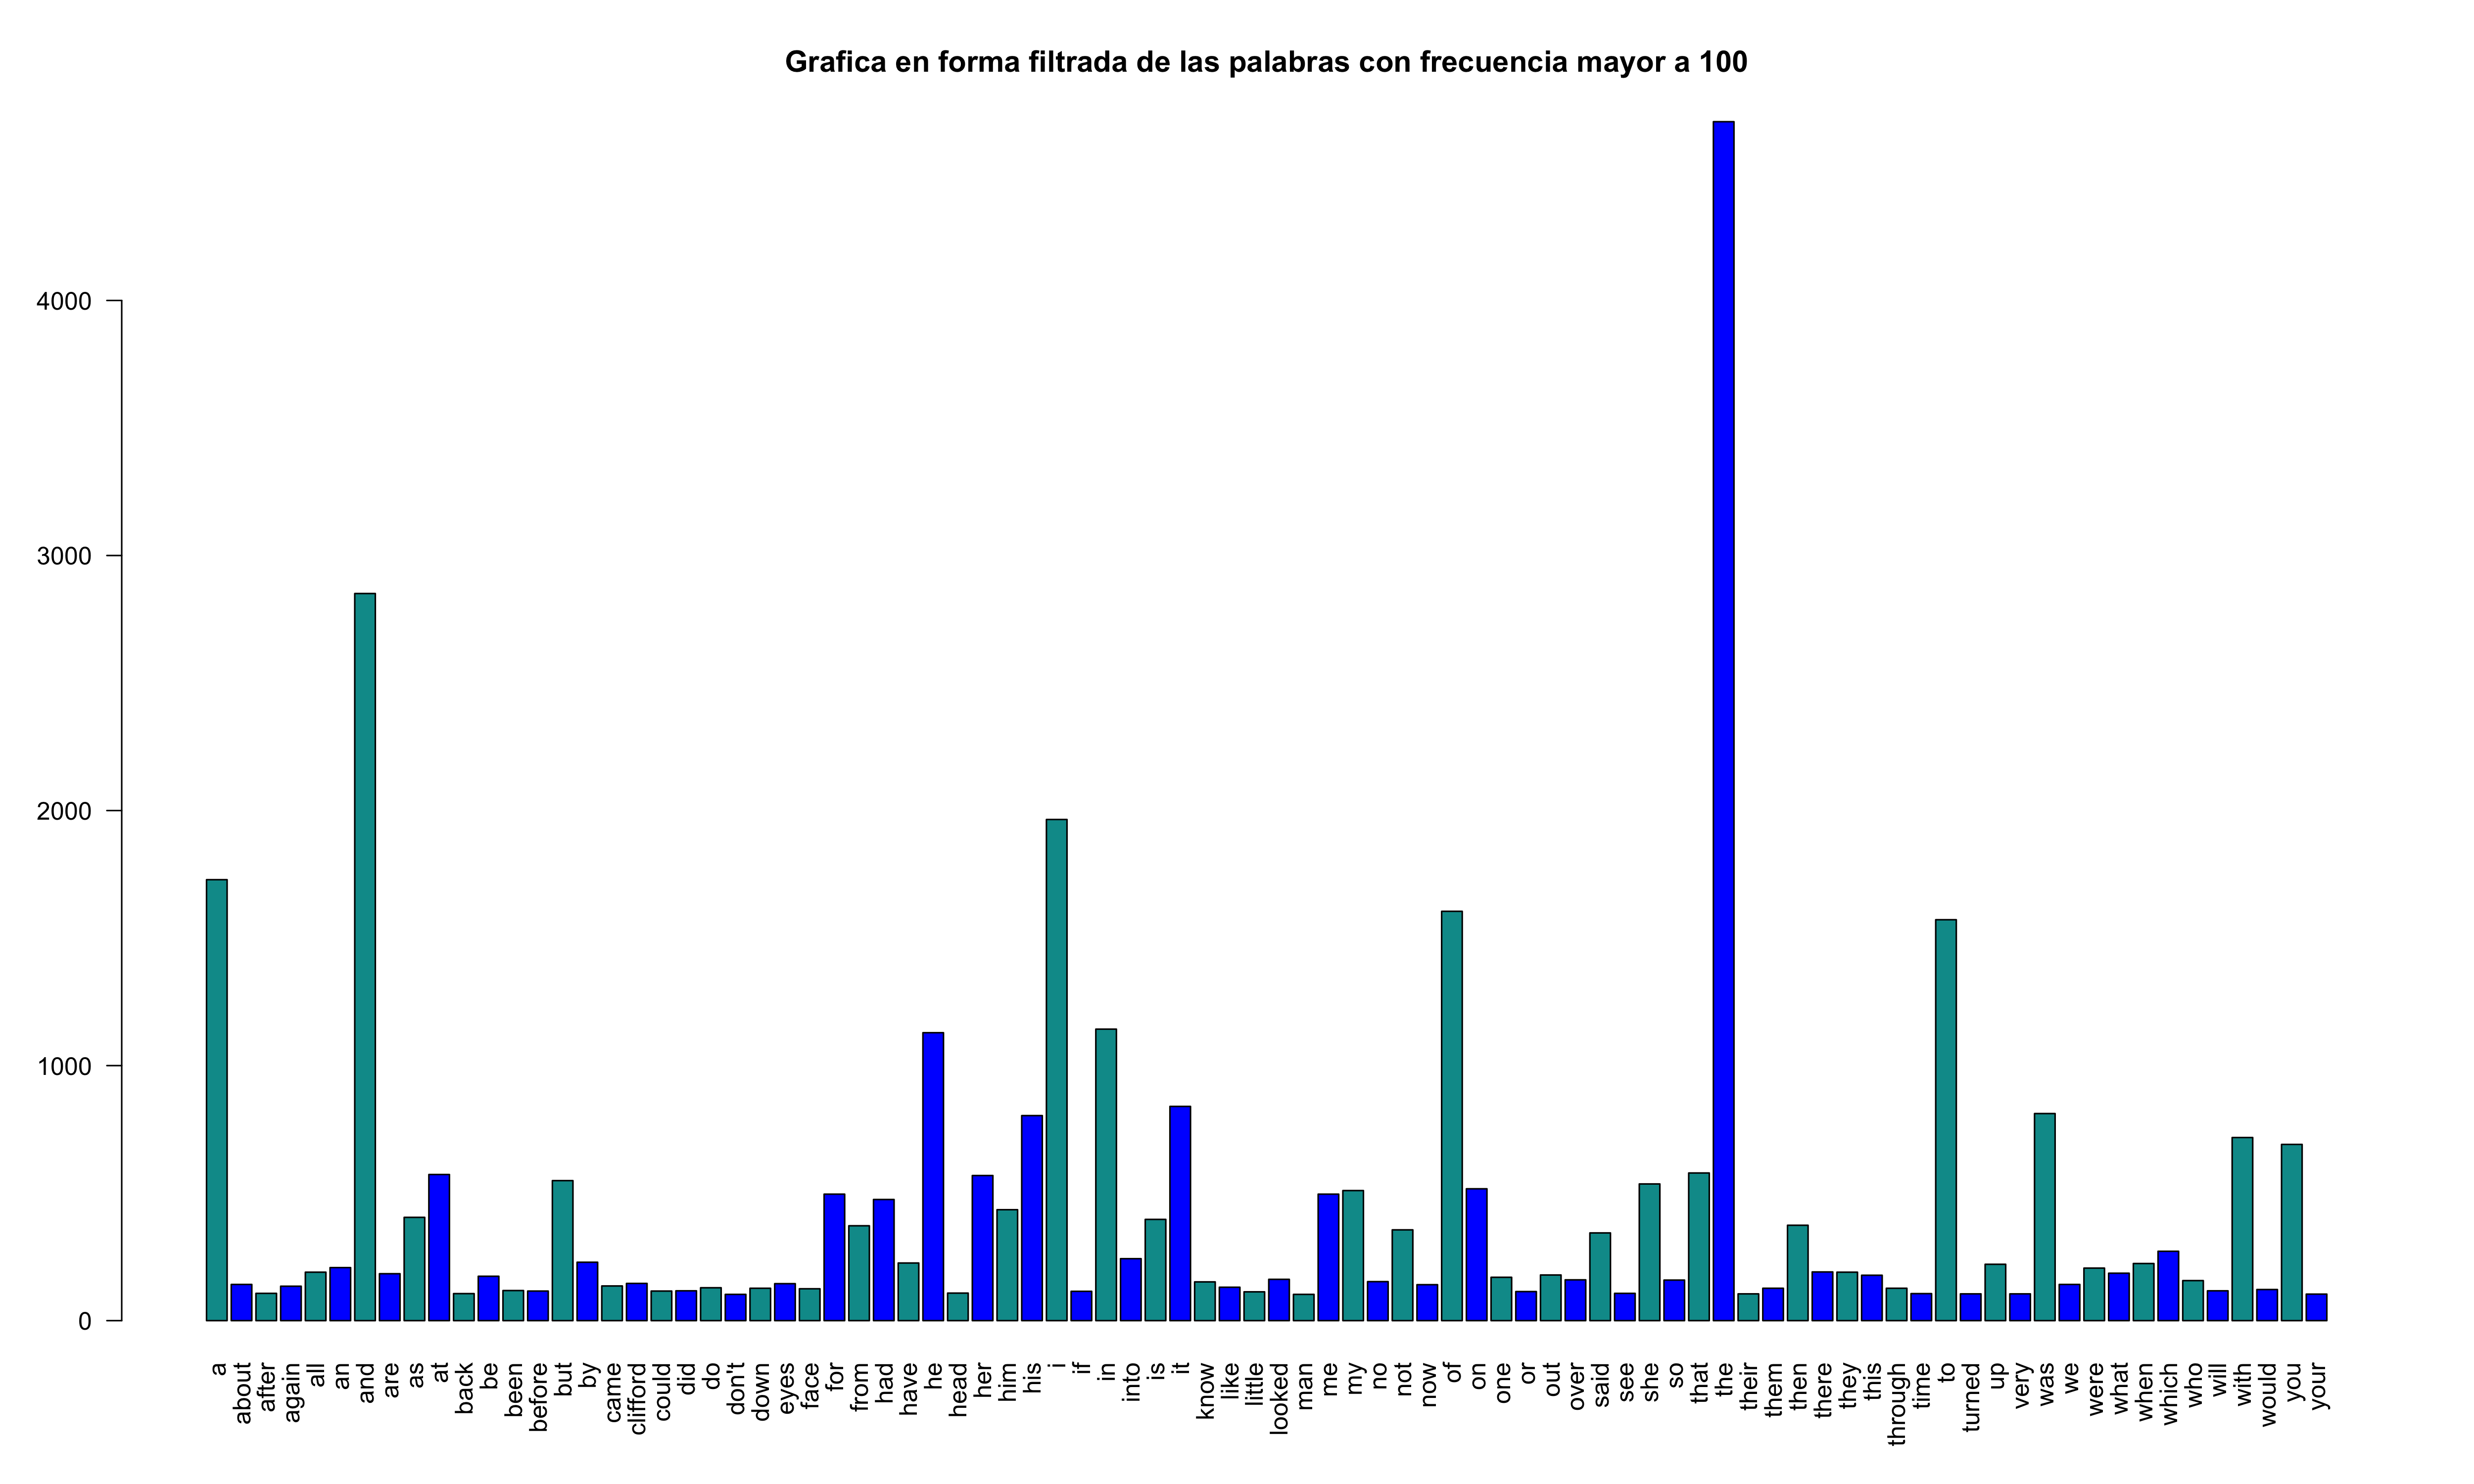
\includegraphics[scale=0.09]{Gráfica_en_forma_filtrada_de_las_palabras_con_frecuencia_mayor_a_100.png}
    \caption{ En esta gráfica se expone el filtrado de palabras mayor a 100.}
    \label{fig:Palabras}
\end{figure}
\begin{figure}[ht]
    \centering
    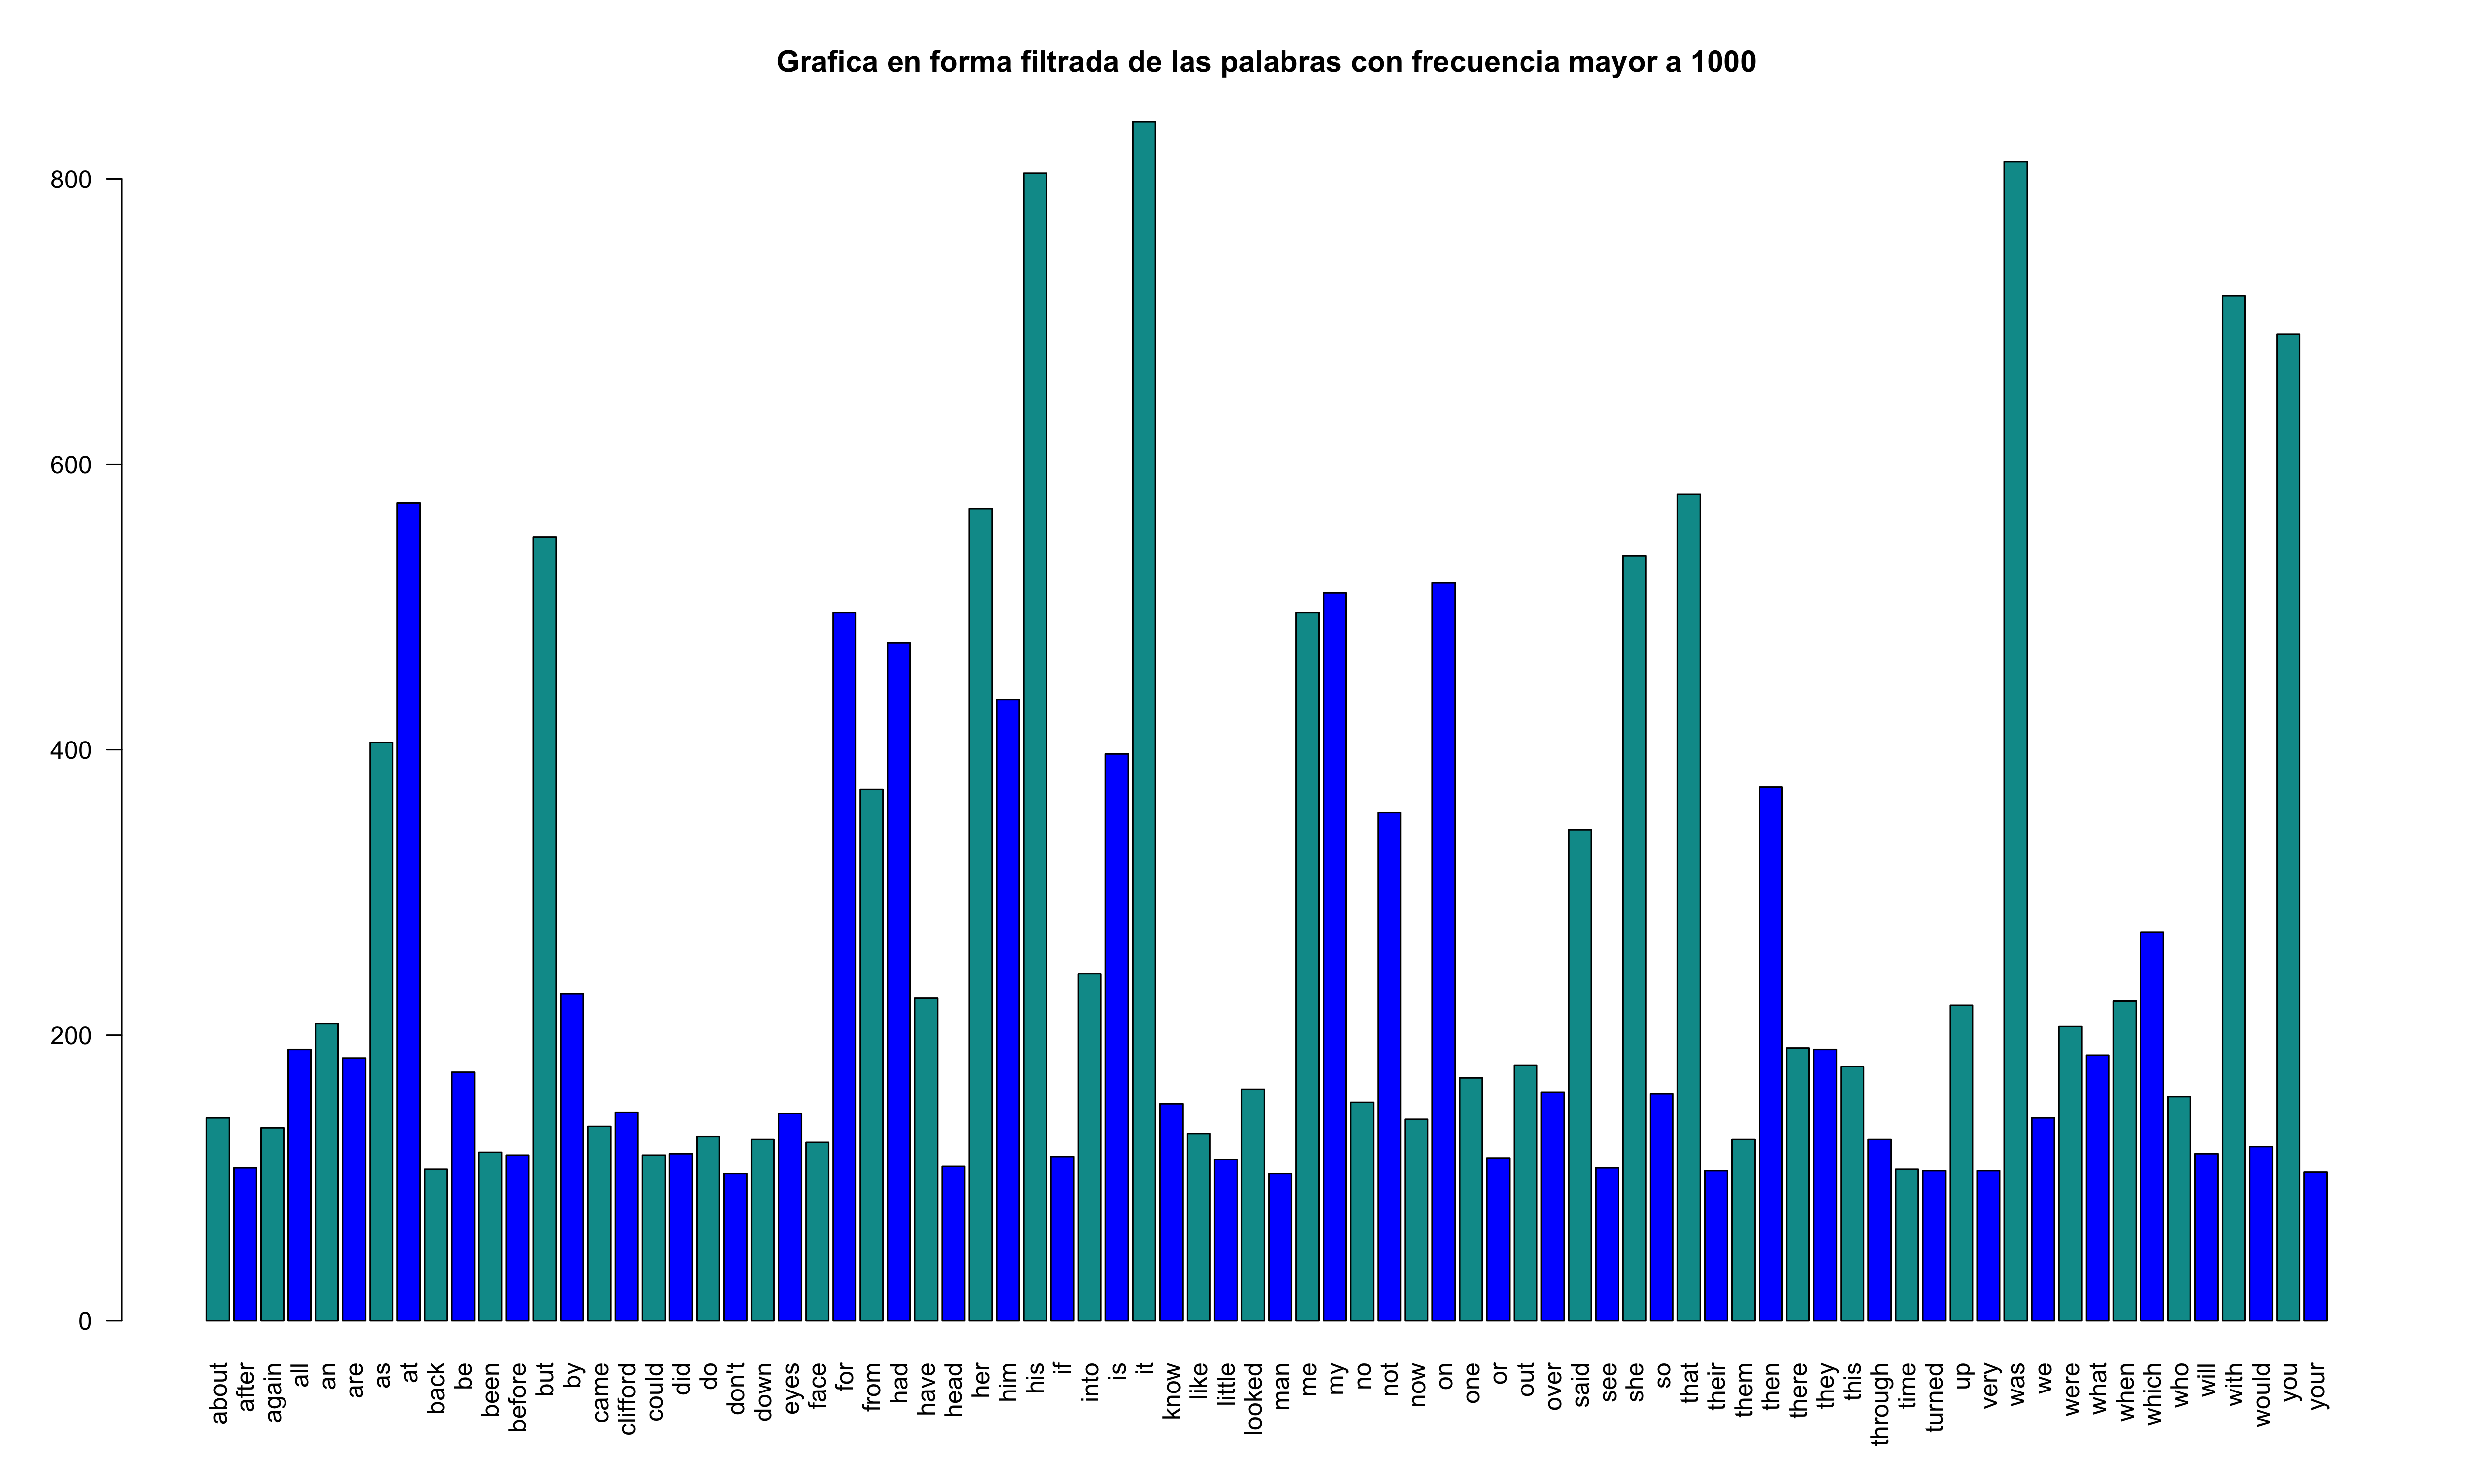
\includegraphics[scale=0.09]{Gráfica_en_forma_filtrada_de_las_palabras_con_frecuencia_mayor_a_1000.png}
    \caption{En esta gráfica se expone el filtrado de palabras mayor a 1000 sin ordenamiento.}
    \label{fig:Palabras}
\end{figure}
\begin{figure}[ht]
    \centering
    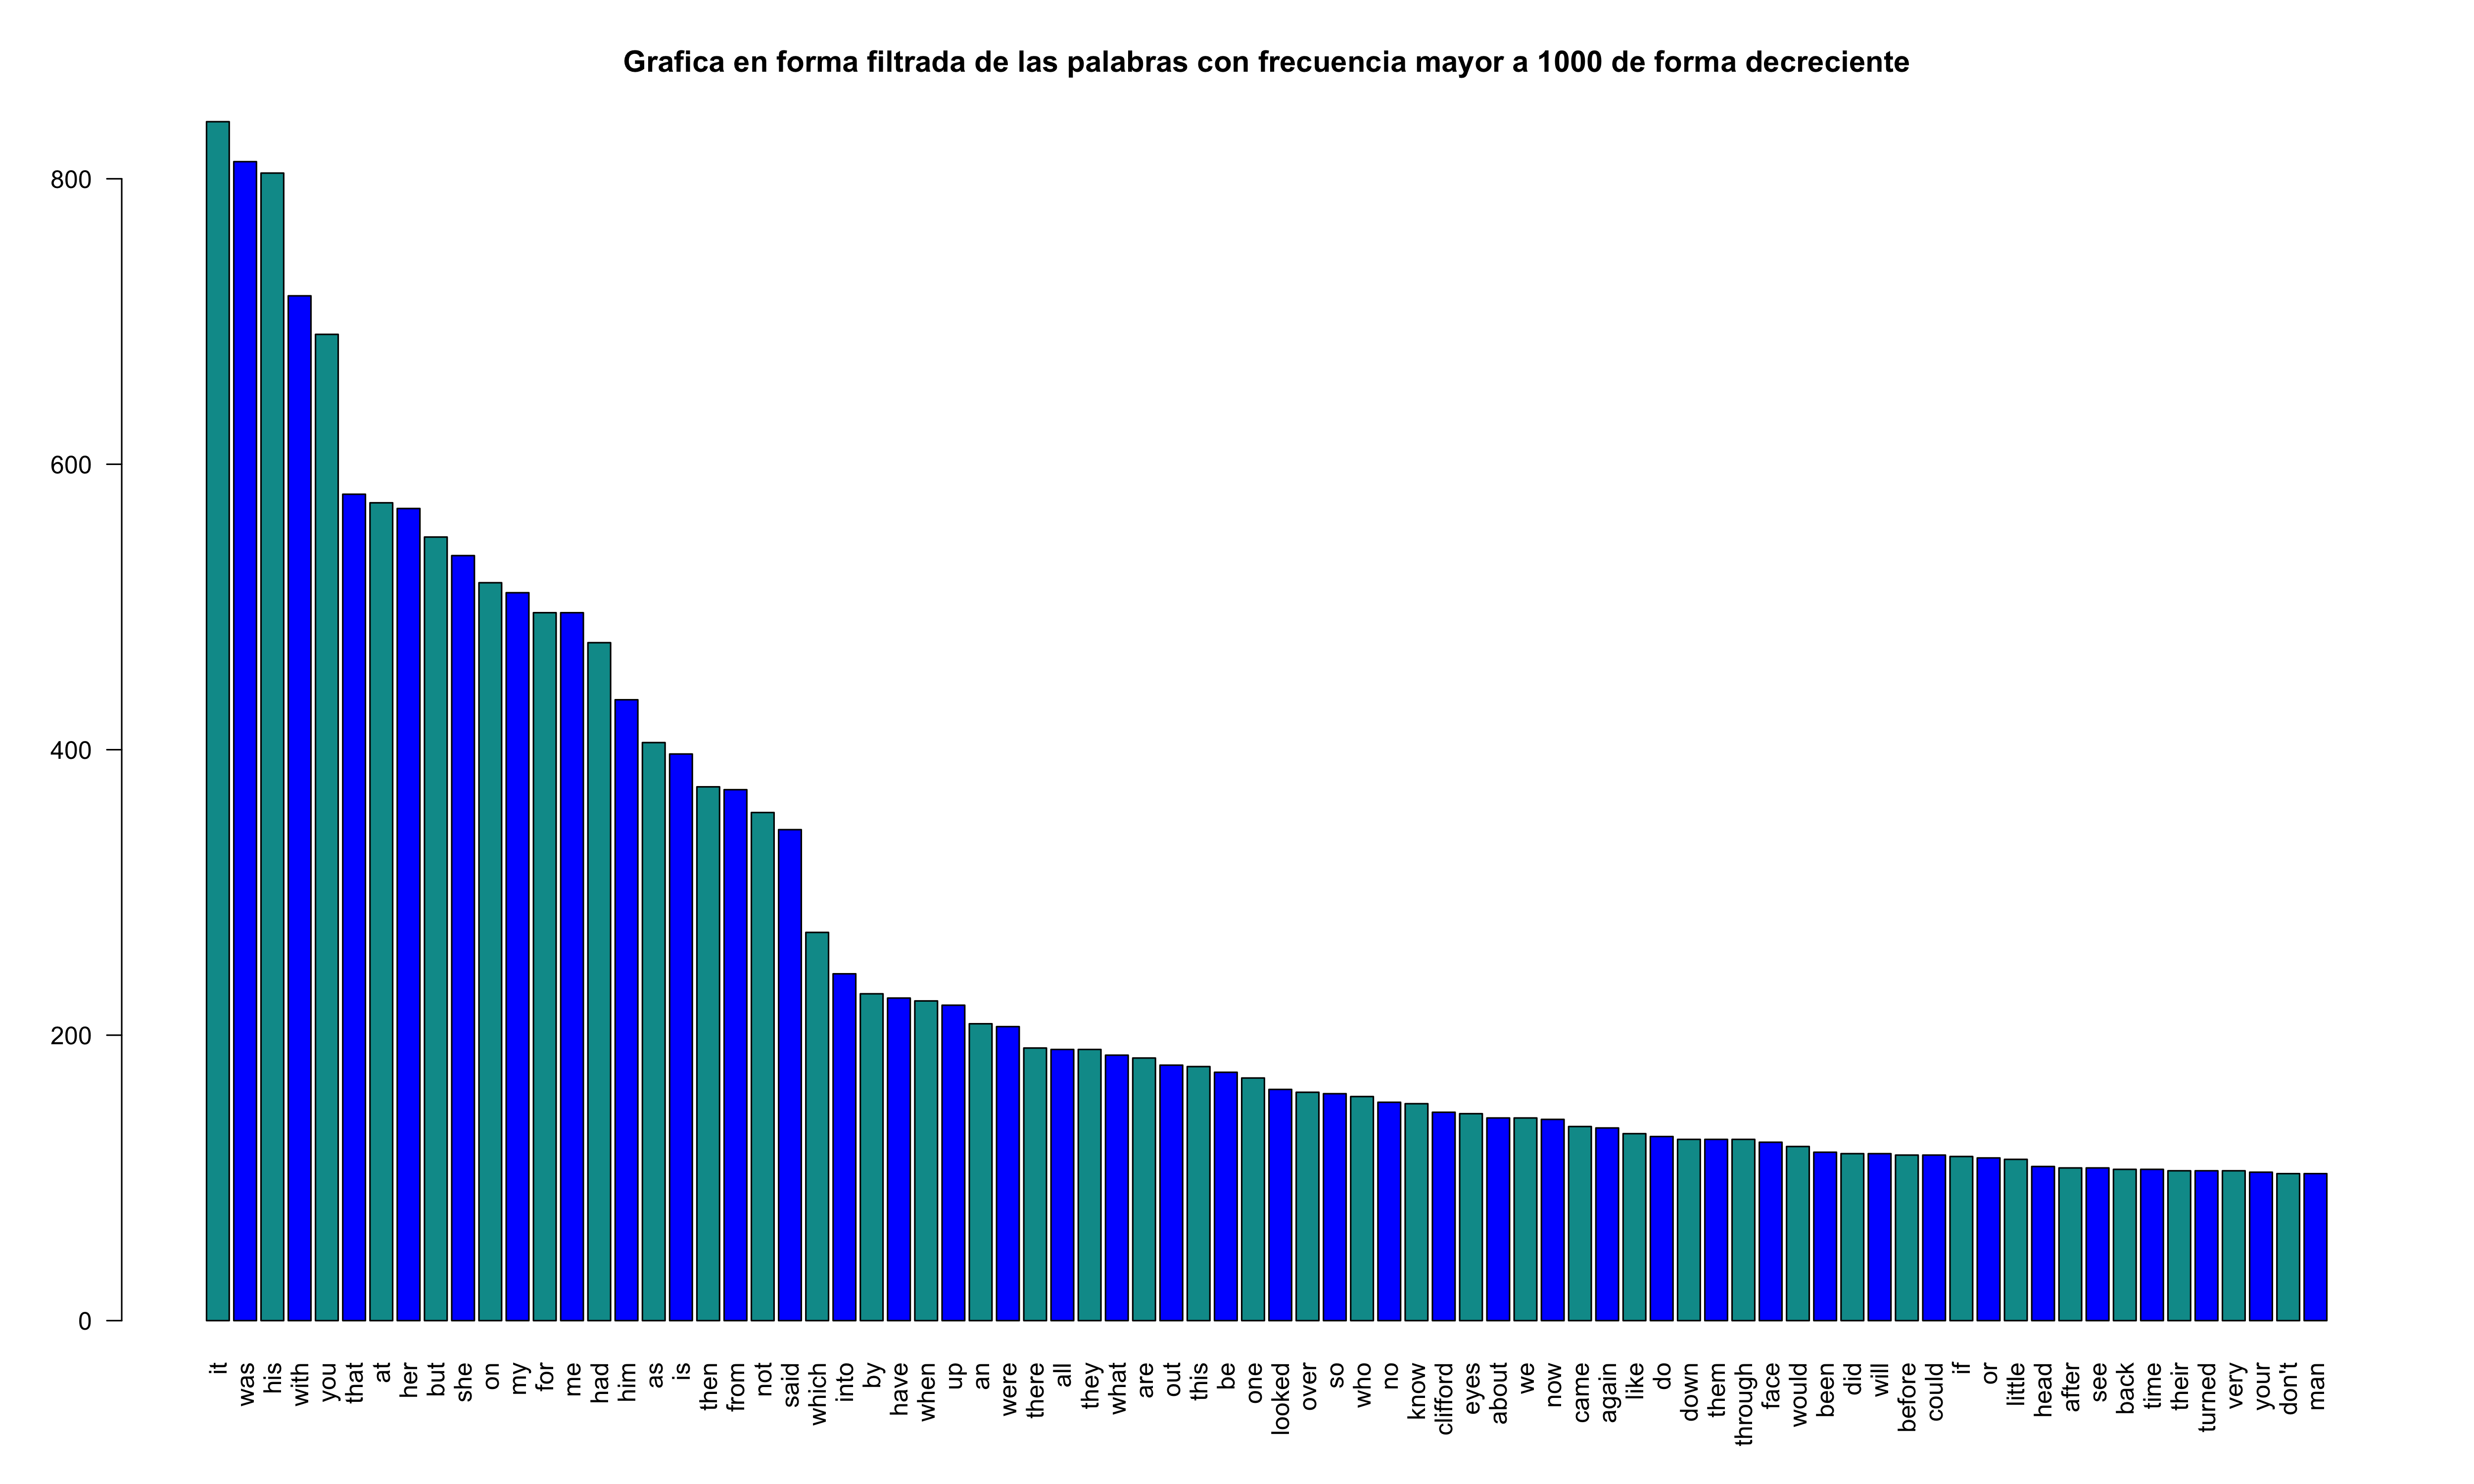
\includegraphics[scale=0.09]{Gráfica_en_forma_filtrada_de_las_palabras_con_frecuencia_mayor_a_1000_de_forma_decreciente.png}
    \caption{En esta gráfica se expone el filtrado de palabras mayor a 1000 de forma ordenada.}
    \label{fig:Palabras}
\end{figure}


\clearpage
\bibliographystyle{plain}
\bibliography{references}
\end{document}
